\begin{center}
	\textbf{Advanced Scan Feedback Questionnaire}\par
	\textbf{Participant No.}\par
\end{center}

\vspace{0.5cm}

\begin{figure}[h]
\begin{center}
	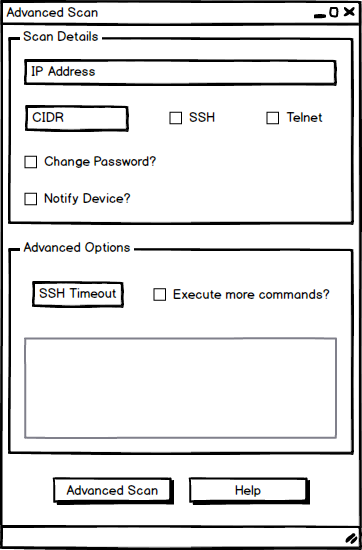
\includegraphics[width=0.5\textwidth]{img/advanced_scan_mockup.png}
\end{center}
\end{figure}

\vspace{0.5cm}

The above image shows the advanced scan window the program will produce upon pressing the \textit{Advanced Scan} button on
the client interface. It shows the same options as the regular quick scan, although with two more options for specifying a
scanning timeout and any extra commands the user wants to send to the device.

\vspace{0.5cm}

\textbf{1.} On a scale from 1 to 10, how clear would you consider the above interface to be?

\begin{center}
	\begin{table}[h]
	\label{my-label}
	\begin{tabularx}{\textwidth}{XXXXXXXXXX}
	\multicolumn{5}{l}{Unclear} & \multicolumn{5}{r}{Clear} \\
	\centering
	1    & 2    & 3    & 4    & 5    & 6   & 7   & 8   & 9  & 10
	\end{tabularx}
	\end{table}
\end{center}

\textbf{2.} Briefly describe how you would perform an advanced scan.

\vspace{5cm}

\textbf{3.} Are there any improvements (additions, changes, removals, etc.) you would make to the current design?

\vspace{5cm}
